\documentclass[tikz,border=0pt]{standalone}

\usepackage[T1]{fontenc}
\usepackage[american]{circuitikz}
\usetikzlibrary{arrows.meta,backgrounds,calc,fit,positioning}

\definecolor{DcPositive}{HTML}{9C2F24}
\definecolor{DcNegative}{HTML}{37474F}
\definecolor{AcPower}{HTML}{1F4E79}
\definecolor{KBusWire}{HTML}{1769AA}
\definecolor{KBatWire}{HTML}{00838F}
\definecolor{MonitorPower}{HTML}{B05A00}
\definecolor{ControlWire}{HTML}{18794E}
\definecolor{DataWire}{HTML}{5E35B1}
\definecolor{FutureWire}{HTML}{7B1FA2}
\definecolor{ModuleFill}{HTML}{F4F7FA}
\definecolor{WarningRed}{HTML}{B3261E}
\definecolor{TapZero}{HTML}{455A64}
\definecolor{TapOne}{HTML}{6D4C41}
\definecolor{TapTwo}{HTML}{2E7D32}
\definecolor{TapThree}{HTML}{1565C0}
\definecolor{TapFour}{HTML}{8E24AA}

\tikzset{
  module body/.style={
    draw=black!75,
    fill=ModuleFill,
    line width=0.9pt,
    rounded corners=2pt,
    inner sep=0pt
  },
  module title/.style={font=\sffamily\bfseries, align=center},
  module port/.style={
    circle,
    draw=black!70,
    line width=0.5pt,
    minimum size=5pt,
    inner sep=0pt
  },
  port label/.style={
    font=\sffamily\tiny\bfseries,
    text=black!80,
    inner sep=0.7pt
  },
  pack enclosure/.style={
    draw=black!55,
    dashed,
    line width=0.8pt,
    rounded corners=3pt
  },
  harness jacket/.style={
    draw=black!35,
    dashed,
    line width=0.7pt,
    rounded corners=2pt
  },
  dc positive/.style={draw=DcPositive, line width=2.3pt},
  dc negative/.style={draw=DcNegative, line width=2.3pt},
  ac power/.style={draw=AcPower, line width=1.8pt},
  k bus/.style={draw=KBusWire, line width=1.0pt},
  k battery/.style={draw=KBatWire, line width=1.0pt},
  monitor power/.style={draw=MonitorPower, line width=1.0pt},
  monitor ground/.style={draw=DcNegative, line width=1.0pt},
  present control/.style={draw=ControlWire, line width=1.0pt},
  data link/.style={
    draw=DataWire,
    dashed,
    line width=1.0pt,
    -{Stealth[length=2.4mm]}
  },
  bidirectional data/.style={
    draw=DataWire,
    dashed,
    line width=1.0pt,
    {Stealth[length=2.4mm]}-{Stealth[length=2.4mm]}
  },
  future link/.style={
    draw=FutureWire,
    dash pattern=on 5pt off 2pt on 1pt off 2pt,
    line width=1.0pt,
    -{Stealth[length=2.4mm]}
  },
  future box/.style={
    draw=FutureWire,
    dash pattern=on 5pt off 2pt on 1pt off 2pt,
    fill=FutureWire!4,
    text=FutureWire,
    line width=0.8pt,
    rounded corners=2pt,
    font=\sffamily\tiny\bfseries,
    align=center,
    inner sep=3pt
  },
  note/.style={font=\sffamily\scriptsize, align=center},
  tiny note/.style={font=\sffamily\tiny, align=center},
  label text/.style={font=\sffamily\small, align=center},
  warning box/.style={
    draw=WarningRed,
    fill=WarningRed!5,
    text=WarningRed,
    line width=0.8pt,
    rounded corners=2pt,
    font=\sffamily\scriptsize\bfseries,
    align=center,
    inner sep=4pt
  },
  state box/.style={
    draw=black!55,
    fill=black!2,
    line width=0.7pt,
    rounded corners=2pt,
    font=\sffamily\tiny,
    align=left,
    inner sep=4pt
  },
  pics/module/.style args={#1/#2/#3}{
    code={
      \node[module body, minimum width=#2, minimum height=#3] (-body) {};
      \node[module title, anchor=north, yshift=-6pt] at (-body.north) {#1};
    }
  }
}

\newcommand{\ModulePort}[5]{%
  \node[module port, fill=#5, label={[port label]#4:{#3}}] (#1) at #2 {};%
}

% Semantic wrappers make the two grouped-but-independent harnesses explicit and
% give repository validation stable invariants to protect.
\newcommand{\BalanceTapPort}[5]{\ModulePort{#1}{#2}{#3}{#4}{#5}}
\newcommand{\ImplementedMonitorPort}[5]{\ModulePort{#1}{#2}{#3}{#4}{#5}}

\ctikzset{
  bipoles/thickness=1.4,
  nodes width=0.08
}

\begin{document}
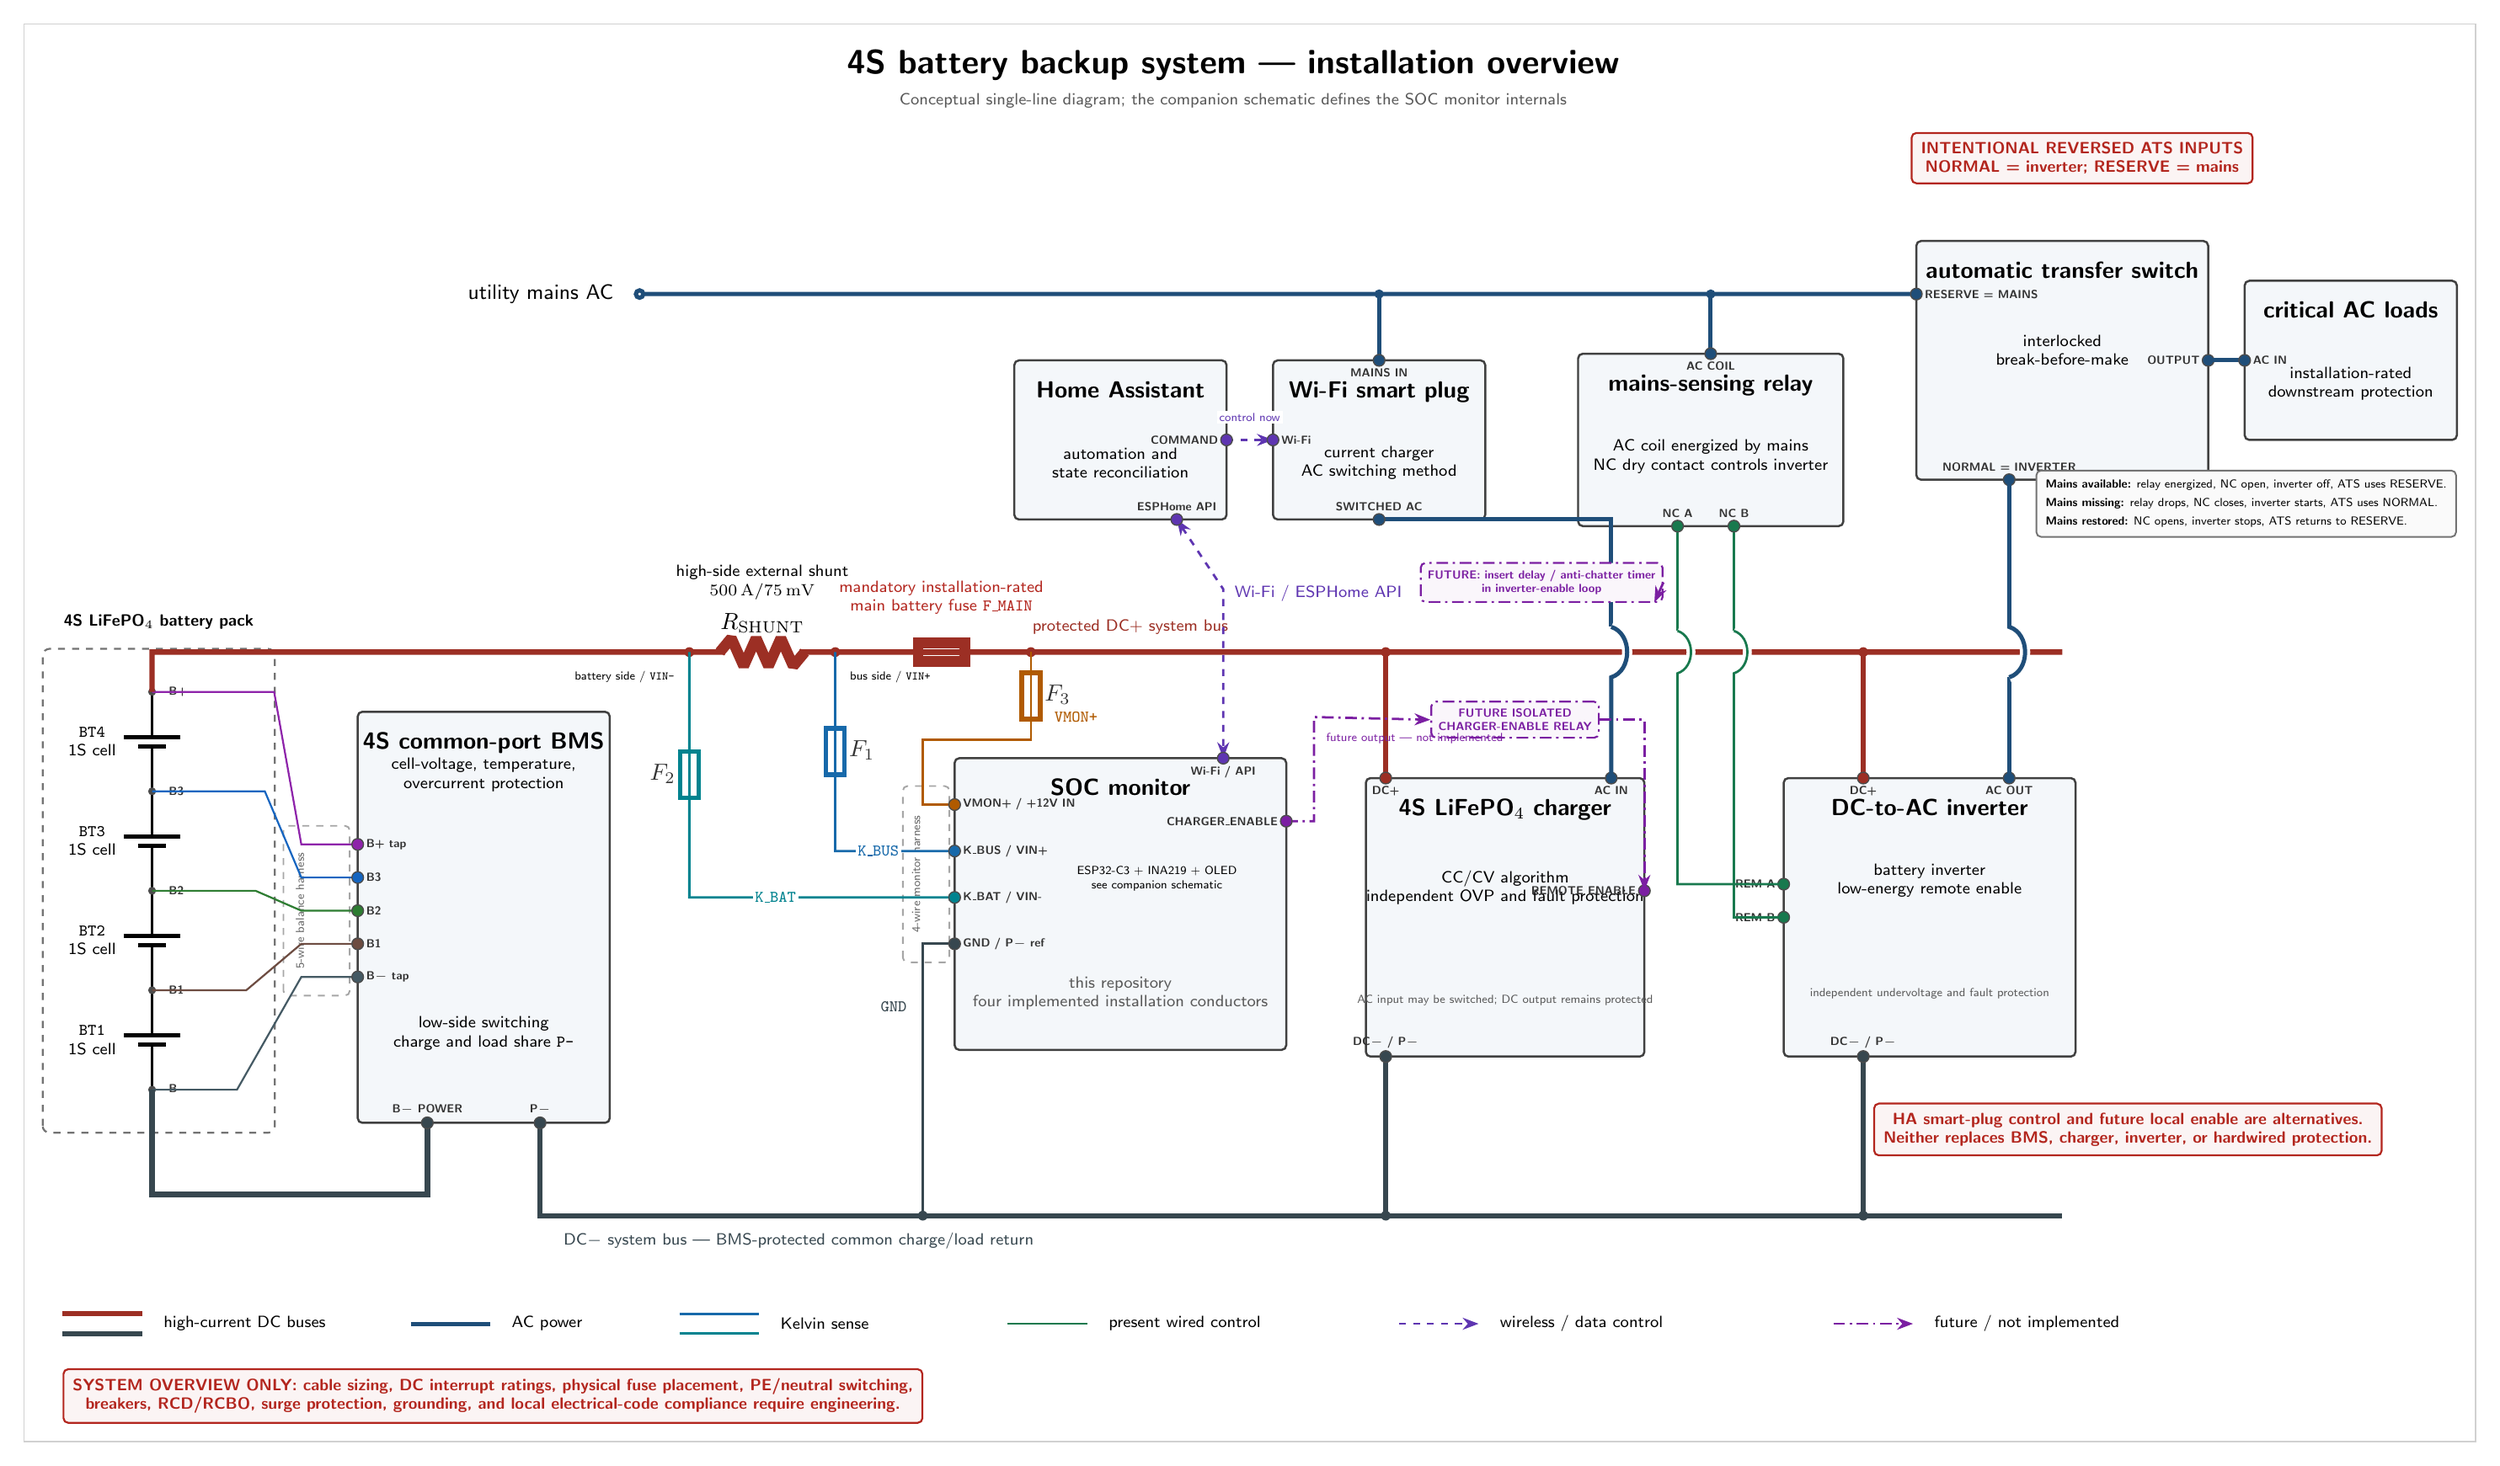
\begin{tikzpicture}[font=\sffamily]
  \begin{scope}[local bounding box=diagram-content]

  % --------------------------------------------------------------------------
  % Title and scope.
  % --------------------------------------------------------------------------
  \node[font=\sffamily\Large\bfseries] at (18.5,18.65)
    {4S battery backup system --- installation overview};
  \node[note, text=black!65] at (18.5,18.12)
    {Conceptual single-line diagram; the companion schematic defines the SOC monitor internals};

  % --------------------------------------------------------------------------
  % Four individual cells inside one dashed battery-pack enclosure. Electrical
  % series links are solid; only the physical grouping boundary is dashed.
  % --------------------------------------------------------------------------
  \draw[pack enclosure] (0.55,2.55) rectangle (4.05,9.85);
  \node[note, font=\sffamily\scriptsize\bfseries, fill=white, inner sep=1pt]
    at (2.30,10.25) {4S LiFePO$_4$ battery pack};

  \draw[line width=0.9pt]
    (2.20,9.20) to[battery1] (2.20,7.70)
    to[battery1] (2.20,6.20)
    to[battery1] (2.20,4.70)
    to[battery1] (2.20,3.20);

  \node[note, anchor=east] at (1.78,8.45) {\texttt{BT4}\\1S cell};
  \node[note, anchor=east] at (1.78,6.95) {\texttt{BT3}\\1S cell};
  \node[note, anchor=east] at (1.78,5.45) {\texttt{BT2}\\1S cell};
  \node[note, anchor=east] at (1.78,3.95) {\texttt{BT1}\\1S cell};

  \foreach \y in {3.20,4.70,6.20,7.70,9.20} {
    \fill[black!70] (2.20,\y) circle (1.7pt);
  }
  \node[port label, anchor=west] at (2.42,3.20) {B$-$};
  \node[port label, anchor=west] at (2.42,4.70) {B1};
  \node[port label, anchor=west] at (2.42,6.20) {B2};
  \node[port label, anchor=west] at (2.42,7.70) {B3};
  \node[port label, anchor=west] at (2.42,9.20) {B+};

  % --------------------------------------------------------------------------
  % Common-port low-side 4S BMS. The five balance leads converge physically as
  % a harness but remain distinct, solid, and traceable end-to-end.
  % --------------------------------------------------------------------------
  \pic (bms) at (7.20,5.80)
    {module={4S common-port BMS/3.8cm/6.2cm}};
  \node[note] at (7.20,7.95)
    {cell-voltage, temperature,\\overcurrent protection};
  \node[note] at (7.20,4.05)
    {low-side switching\\charge and load share \texttt{P-}};

  \draw[harness jacket] (4.18,4.62) rectangle (5.18,7.18);
  \node[tiny note, text=black!60, rotate=90] at (4.43,5.90)
    {5-wire balance harness};

  \draw[draw=TapZero, line width=0.8pt]
    (2.20,3.20) -- (3.48,3.20) -- (4.45,4.90) -- (5.30,4.90);
  \draw[draw=TapOne, line width=0.8pt]
    (2.20,4.70) -- (3.62,4.70) -- (4.45,5.40) -- (5.30,5.40);
  \draw[draw=TapTwo, line width=0.8pt]
    (2.20,6.20) -- (3.76,6.20) -- (4.45,5.90) -- (5.30,5.90);
  \draw[draw=TapThree, line width=0.8pt]
    (2.20,7.70) -- (3.90,7.70) -- (4.45,6.40) -- (5.30,6.40);
  \draw[draw=TapFour, line width=0.8pt]
    (2.20,9.20) -- (4.04,9.20) -- (4.45,6.90) -- (5.30,6.90);

  \BalanceTapPort{bms-tap-bminus}{(5.30,4.90)}{B$-$ tap}{right}{TapZero}
  \BalanceTapPort{bms-tap-b1}{(5.30,5.40)}{B1}{right}{TapOne}
  \BalanceTapPort{bms-tap-b2}{(5.30,5.90)}{B2}{right}{TapTwo}
  \BalanceTapPort{bms-tap-b3}{(5.30,6.40)}{B3}{right}{TapThree}
  \BalanceTapPort{bms-tap-bplus}{(5.30,6.90)}{B+ tap}{right}{TapFour}

  % BMS high-current negative path and protected system return bus.
  \draw[dc negative]
    (2.20,3.20) -- (2.20,1.62) -- (6.35,1.62) -- (6.35,2.70);
  \draw[dc negative]
    (8.05,2.70) -- (8.05,1.30) -- (31.00,1.30);
  \ModulePort{bms-power-bminus}{(6.35,2.70)}{B$-$ POWER}{above}{DcNegative}
  \ModulePort{bms-power-pminus}{(8.05,2.70)}{P$-$}{above}{DcNegative}
  \node[note, text=DcNegative, anchor=west] at (8.28,0.92)
    {DC$-$ system bus --- BMS-protected common charge/load return};

  % --------------------------------------------------------------------------
  % Positive high-current path: battery -> shunt -> main fuse -> protected bus.
  % --------------------------------------------------------------------------
  \draw[dc positive]
    (2.20,9.20) -- (2.20,9.80) -- (10.30,9.80)
    to[R, l^={$R_{\mathrm{SHUNT}}$}] (12.50,9.80)
    -- (13.10,9.80) to[fuse] (15.10,9.80)
    -- (31.00,9.80);
  \fill[DcPositive] (10.30,9.80) circle (2.1pt);
  \fill[DcPositive] (12.50,9.80) circle (2.1pt);

  \node[note] at (11.40,10.85)
    {high-side external shunt\\$500\,\mathrm{A}/75\,\mathrm{mV}$};
  \node[tiny note, anchor=east] at (10.20,9.42)
    {battery side / \texttt{VIN-}};
  \node[tiny note, anchor=west] at (12.60,9.42)
    {bus side / \texttt{VIN+}};
  \node[note, text=WarningRed] at (14.10,10.62)
    {mandatory installation-rated\\main battery fuse \texttt{F\_MAIN}};
  \node[note, text=DcPositive, anchor=west] at (15.35,10.18)
    {protected DC+ system bus};

  % --------------------------------------------------------------------------
  % The repository implementation is one module at installation level. Four
  % logical conductors form one physical harness without electrical joining.
  % --------------------------------------------------------------------------
  \pic (monitor) at (16.80,6.00)
    {module={SOC monitor/5.0cm/4.4cm}};
  \node[tiny note] at (17.35,6.38)
    {ESP32-C3 + INA219 + OLED\\see companion schematic};
  \node[note, text=black!65] at (16.80,4.65)
    {this repository\\four implemented installation conductors};

  \draw[harness jacket] (13.52,5.12) rectangle (14.22,7.78);
  \node[tiny note, text=black!60, rotate=90] at (13.72,6.45)
    {4-wire monitor harness};

  % K_BAT: battery-side differential input through F2.
  \draw[k battery]
    (10.30,9.80) to[fuse, l_={\textcolor{black!80}{$F_2$}}] (10.30,6.10)
    -- (14.30,6.10);
  \node[note, text=KBatWire, fill=white, inner sep=1pt] at (11.60,6.10)
    {\texttt{K\_BAT}};

  % K_BUS: bus-side differential input through F1.
  \draw[k bus]
    (12.50,9.80) to[fuse, l={\textcolor{black!80}{$F_1$}}] (12.50,6.80)
    -- (14.30,6.80);
  \node[note, text=KBusWire, fill=white, inner sep=1pt] at (13.15,6.80)
    {\texttt{K\_BUS}};

  % VMON+: independent protected monitor supply input through F3.
  \fill[DcPositive] (15.45,9.80) circle (2.1pt);
  \draw[monitor power]
    (15.45,9.80) to[fuse, l={\textcolor{black!80}{$F_3$}}] (15.45,8.48)
    -- (13.82,8.48) -- (13.82,7.50) -- (14.30,7.50);
  \node[note, text=MonitorPower, anchor=west] at (15.68,8.82)
    {\texttt{VMON+}};

  % GND: non-isolated reference and supply return on the BMS P- side.
  \fill[DcNegative] (13.82,1.30) circle (2.1pt);
  \draw[monitor ground]
    (13.82,1.30) -- (13.82,5.40) -- (14.30,5.40);
  \node[note, text=DcNegative, anchor=east, fill=white, inner sep=1pt]
    at (13.62,4.45) {\texttt{GND}};

  \ImplementedMonitorPort{monitor-vmon}{(14.30,7.50)}{VMON+ / +12V IN}{right}{MonitorPower}
  \ImplementedMonitorPort{monitor-kbus}{(14.30,6.80)}{K\_BUS / VIN+}{right}{KBusWire}
  \ImplementedMonitorPort{monitor-kbat}{(14.30,6.10)}{K\_BAT / VIN-}{right}{KBatWire}
  \ImplementedMonitorPort{monitor-gnd}{(14.30,5.40)}{GND / P$-$ ref}{right}{DcNegative}

  % --------------------------------------------------------------------------
  % Charger and inverter share the protected DC buses.
  % --------------------------------------------------------------------------
  \pic (charger) at (22.60,5.80)
    {module={4S LiFePO$_4$ charger/4.2cm/4.2cm}};
  \node[note] at (22.60,6.25)
    {CC/CV algorithm\\independent OVP and fault protection};
  \node[tiny note, text=black!65] at (22.60,4.55)
    {AC input may be switched; DC output remains protected};

  \pic (inverter) at (29.00,5.80)
    {module={DC-to-AC inverter/4.4cm/4.2cm}};
  \node[note] at (29.00,6.35)
    {battery inverter\\low-energy remote enable};
  \node[tiny note, text=black!65] at (29.00,4.65)
    {independent undervoltage and fault protection};

  % Intended DC connections.
  \fill[DcPositive] (20.80,9.80) circle (2.1pt);
  \draw[dc positive] (20.80,9.80) -- (20.80,7.90);
  \fill[DcNegative] (20.80,1.30) circle (2.1pt);
  \draw[dc negative] (20.80,1.30) -- (20.80,3.70);

  \fill[DcPositive] (28.00,9.80) circle (2.1pt);
  \draw[dc positive] (28.00,9.80) -- (28.00,7.90);
  \fill[DcNegative] (28.00,1.30) circle (2.1pt);
  \draw[dc negative] (28.00,1.30) -- (28.00,3.70);

  \ModulePort{charger-dc-plus}{(20.80,7.90)}{DC+}{below}{DcPositive}
  \ModulePort{charger-ac-in}{(24.20,7.90)}{AC IN}{below}{AcPower}
  \ModulePort{charger-dc-minus}{(20.80,3.70)}{DC$-$ / P$-$}{above}{DcNegative}
  \ModulePort{charger-remote}{(24.70,6.20)}{REMOTE ENABLE}{left}{FutureWire}

  \ModulePort{inverter-dc-plus}{(28.00,7.90)}{DC+}{below}{DcPositive}
  \ModulePort{inverter-ac-out}{(30.20,7.90)}{AC OUT}{below}{AcPower}
  \ModulePort{inverter-dc-minus}{(28.00,3.70)}{DC$-$ / P$-$}{above}{DcNegative}
  \ModulePort{inverter-remote-a}{(26.80,6.30)}{REM A}{left}{ControlWire}
  \ModulePort{inverter-remote-b}{(26.80,5.80)}{REM B}{left}{ControlWire}

  % --------------------------------------------------------------------------
  % Upper AC lane: utility mains, current smart-plug charger control, mains
  % sensing relay, intentionally reversed ATS inputs, and critical loads.
  % --------------------------------------------------------------------------
  \draw[ac power]
    (9.55,15.20) to[short, o-] (28.80,15.20);
  \node[label text, anchor=east] at (9.28,15.20)
    {utility mains AC};

  \pic (homeassistant) at (16.80,13.00)
    {module={Home Assistant/3.2cm/2.4cm}};
  \node[note] at (16.80,12.65)
    {automation and\\state reconciliation};

  \pic (smartplug) at (20.70,13.00)
    {module={Wi-Fi smart plug/3.2cm/2.4cm}};
  \node[note] at (20.70,12.65)
    {current charger\\AC switching method};

  \pic (mainsrelay) at (25.70,13.00)
    {module={mains-sensing relay/4.0cm/2.6cm}};
  \node[note] at (25.70,12.75)
    {AC coil energized by mains\\NC dry contact controls inverter};

  \pic (ats) at (31.00,14.20)
    {module={automatic transfer switch/4.4cm/3.6cm}};
  \node[note] at (31.00,14.35)
    {interlocked\\break-before-make};

  \pic (loads) at (35.35,14.20)
    {module={critical AC loads/3.2cm/2.4cm}};
  \node[note] at (35.35,13.85)
    {installation-rated\\downstream protection};

  % Mains branches to the current charger switch and sensing-relay coil.
  \fill[AcPower] (20.70,15.20) circle (2.0pt);
  \draw[ac power] (20.70,15.20) -- (20.70,14.20);
  \fill[AcPower] (25.70,15.20) circle (2.0pt);
  \draw[ac power] (25.70,15.20) -- (25.70,14.30);

  % Smart-plug output to charger AC input. A bridge makes the DC+ crossing
  % explicitly non-connecting.
  \draw[ac power]
    (20.70,11.80) -- (24.20,11.80) -- (24.20,10.18);
  \draw[white, line width=4.4pt]
    (24.20,10.18) .. controls (24.52,10.08) and (24.52,9.52) .. (24.20,9.42);
  \draw[ac power]
    (24.20,10.18) .. controls (24.52,10.08) and (24.52,9.52) .. (24.20,9.42)
    -- (24.20,7.90);

  \ModulePort{smartplug-ac-in}{(20.70,14.20)}{MAINS IN}{below}{AcPower}
  \ModulePort{smartplug-ac-out}{(20.70,11.80)}{SWITCHED AC}{above}{AcPower}
  \ModulePort{mainsrelay-coil}{(25.70,14.30)}{AC COIL}{below}{AcPower}

  % ATS reserve is intentionally utility mains, while inverter is NORMAL.
  \ModulePort{ats-reserve}{(28.80,15.20)}{RESERVE = MAINS}{right}{AcPower}
  \ModulePort{ats-normal}{(30.20,12.40)}{NORMAL = INVERTER}{above}{AcPower}
  \ModulePort{ats-output}{(33.20,14.20)}{OUTPUT}{left}{AcPower}
  \draw[ac power] (33.20,14.20) -- (33.75,14.20);
  \ModulePort{loads-input}{(33.75,14.20)}{AC IN}{right}{AcPower}

  % Inverter AC output rises to ATS NORMAL. The curved bridge crosses DC+
  % without an electrical junction.
  \draw[ac power] (30.20,7.90) -- (30.20,9.42);
  \draw[white, line width=4.4pt]
    (30.20,9.42) .. controls (30.52,9.52) and (30.52,10.08) .. (30.20,10.18);
  \draw[ac power]
    (30.20,9.42) .. controls (30.52,9.52) and (30.52,10.08) .. (30.20,10.18)
    -- (30.20,12.40);

  \node[warning box] at (31.30,17.25)
    {INTENTIONAL REVERSED ATS INPUTS\\NORMAL = inverter; RESERVE = mains};

  \node[state box, anchor=north east] at (36.95,12.55)
    {\textbf{Mains available:} relay energized, NC open, inverter off, ATS uses RESERVE.\\[2pt]
     \textbf{Mains missing:} relay drops, NC closes, inverter starts, ATS uses NORMAL.\\[2pt]
     \textbf{Mains restored:} NC opens, inverter stops, ATS returns to RESERVE.};

  % --------------------------------------------------------------------------
  % Present inverter-enable wiring and optional future anti-chatter timer.
  % A two-wire path makes the dry-contact nature explicit.
  % --------------------------------------------------------------------------
  \draw[present control]
    (25.20,11.70) -- (25.20,10.12);
  \draw[white, line width=3.8pt]
    (25.20,10.12) .. controls (25.47,10.03) and (25.47,9.57) .. (25.20,9.48);
  \draw[present control]
    (25.20,10.12) .. controls (25.47,10.03) and (25.47,9.57) .. (25.20,9.48)
    -- (25.20,6.30) -- (26.80,6.30);

  \draw[present control]
    (26.05,11.70) -- (26.05,10.12);
  \draw[white, line width=3.8pt]
    (26.05,10.12) .. controls (26.32,10.03) and (26.32,9.57) .. (26.05,9.48);
  \draw[present control]
    (26.05,10.12) .. controls (26.32,10.03) and (26.32,9.57) .. (26.05,9.48)
    -- (26.05,5.80) -- (26.80,5.80);

  \ModulePort{mainsrelay-nc-a}{(25.20,11.70)}{NC A}{above}{ControlWire}
  \ModulePort{mainsrelay-nc-b}{(26.05,11.70)}{NC B}{above}{ControlWire}

  \node[future box] (timer) at (23.15,10.85)
    {FUTURE: insert delay / anti-chatter timer\\in inverter-enable loop};
  \draw[future link] (timer.east) -- (24.85,10.55);

  % --------------------------------------------------------------------------
  % Current Home Assistant charger control and a separate future local option.
  % --------------------------------------------------------------------------
  \draw[bidirectional data]
    (17.65,11.80) -- (18.35,10.75) -- (18.35,8.20);
  \node[note, text=DataWire, anchor=west, fill=white, inner sep=1pt]
    at (18.48,10.68) {Wi-Fi / ESPHome API};

  \draw[data link] (18.40,13.00) -- (19.10,13.00);
  \node[tiny note, text=DataWire, fill=white, inner sep=1pt]
    at (18.75,13.34) {control now};

  \ModulePort{monitor-wifi}{(18.35,8.20)}{Wi-Fi / API}{below}{DataWire}
  \ModulePort{ha-api}{(17.65,11.80)}{ESPHome API}{above}{DataWire}
  \ModulePort{ha-smartplug}{(18.40,13.00)}{COMMAND}{left}{DataWire}
  \ModulePort{smartplug-control}{(19.10,13.00)}{Wi-Fi}{right}{DataWire}

  % Future local charger control is deliberately outside the implemented
  % four-conductor monitor interface and is an alternative to HA switching.
  \node[future box] (chargerrelay) at (22.75,8.78)
    {FUTURE ISOLATED\\CHARGER-ENABLE RELAY};
  \draw[future link]
    (19.30,7.25) -- (19.72,7.25) -- (19.72,8.82) -- (chargerrelay.west);
  \draw[future link]
    (chargerrelay.east) -- (24.70,8.78) -- (24.70,6.20);
  \ModulePort{monitor-charger-enable}{(19.30,7.25)}{CHARGER\_ENABLE}{left}{FutureWire}
  \node[tiny note, text=FutureWire, anchor=west] at (19.78,8.50)
    {future output --- not implemented};

  \node[warning box, anchor=west] at (28.15,2.60)
    {HA smart-plug control and future local enable are alternatives.\\
     Neither replaces BMS, charger, inverter, or hardwired protection.};

  % --------------------------------------------------------------------------
  % Legend and installation boundary.
  % --------------------------------------------------------------------------
  \draw[dc positive] (0.85,-0.18) -- (2.05,-0.18);
  \draw[dc negative] (0.85,-0.48) -- (2.05,-0.48);
  \node[note, anchor=west] at (2.25,-0.33) {high-current DC buses};

  \draw[ac power] (6.10,-0.33) -- (7.30,-0.33);
  \node[note, anchor=west] at (7.50,-0.33) {AC power};

  \draw[k bus] (10.15,-0.18) -- (11.35,-0.18);
  \draw[k battery] (10.15,-0.48) -- (11.35,-0.48);
  \node[note, anchor=west] at (11.55,-0.33) {Kelvin sense};

  \draw[present control] (15.10,-0.33) -- (16.30,-0.33);
  \node[note, anchor=west] at (16.50,-0.33) {present wired control};

  \draw[data link] (21.00,-0.33) -- (22.20,-0.33);
  \node[note, anchor=west] at (22.40,-0.33) {wireless / data control};

  \draw[future link] (27.55,-0.33) -- (28.75,-0.33);
  \node[note, anchor=west] at (28.95,-0.33) {future / not implemented};

  \node[warning box, anchor=west] at (0.85,-1.42)
    {SYSTEM OVERVIEW ONLY: cable sizing, DC interrupt ratings, physical fuse placement, PE/neutral switching,\\
     breakers, RCD/RCBO, surge protection, grounding, and local electrical-code compliance require engineering.};

  \end{scope}

  % Opaque content-sized canvas for reliable contrast in light and dark viewers.
  \begin{scope}[on background layer]
    \node[
      fill=white,
      draw=black!18,
      line width=0.6pt,
      fit=(diagram-content),
      inner sep=8pt
    ] {};
  \end{scope}
\end{tikzpicture}
\end{document}
